\subsection{Riflessi dell'innovazione tecnologica sulla disciplina giuridica delle TLC}

\begin{figure}
    \centering
    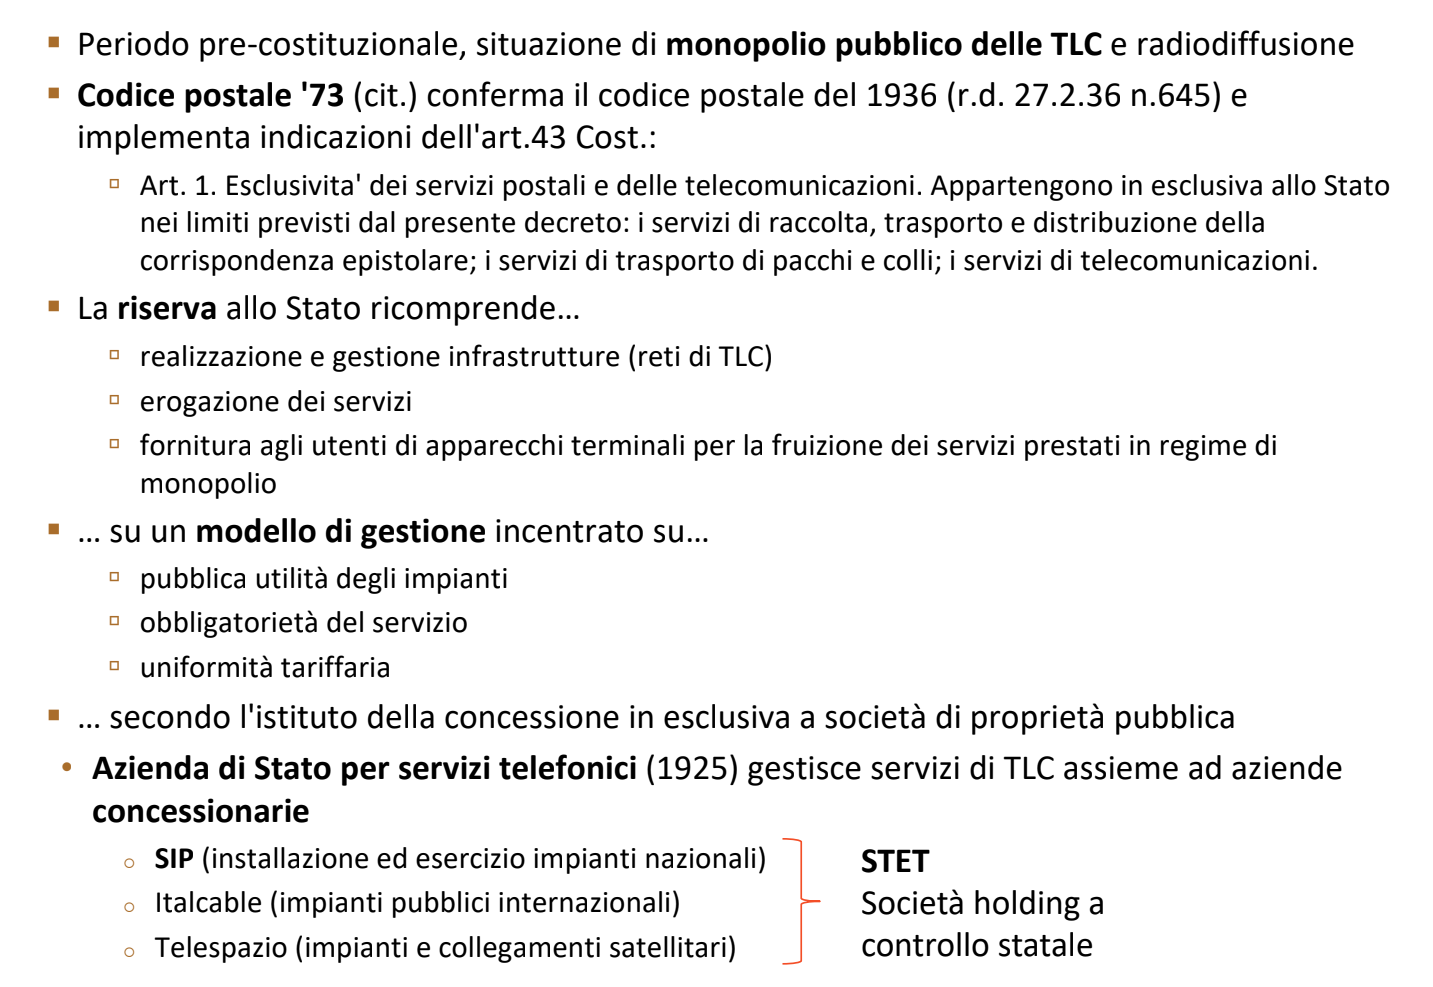
\includegraphics[width=\textwidth]{innovazione tecnologica.png}
\end{figure}


Essendo le problematiche sempre più internazionali (tenendo conto anche della globalizzazione e della mobilità delle persone e delle merci), sempre più decisioni fondamentali vennero prese in sede comunitaria a livello europeo sovranazionale. 

A partire dalla sentenza della Corte di Giustizia del 20/03/1985 su ricorso della Repubblica Italiana vs CE in merito a una sanzione per abuso di posizione dominante a British Telecom ove si respinge il ricorso, si afferma il principio in base al quale le regole della concorrenza sono applicabili anche a organismi pubblici titolari dei diritti esclusivi sulla gestione della rete di telefonia e dei relativi servizi. Ne consegue lo sviluppo di una nuova politica delle TLC a livello europeo volta a:
\begin{itemize}
    \item Liberalizzare i mercati nazionali
    \item Armonizzare le nuove legislazioni nazionali
\end{itemize}

Il processo di regolamentazione comunitaria inizia con il Libro Verde nel 1987 (libro verde sullo sviluppo di un mercato comune dei servizi ed apparati di telecomunicazioni): questo libro trattava della conservazione dei monopoli delle infrastrutture di TLC e della telefonia locale e della liberalizzazione di tutti gli altri servizi. 


ART. 100: sullo stile che la Comunità Europea si dà per cercare di armonizzare e avvicinare i sistemi giuridici dei vari Paesi. 


MAASTRICHT 
ART. 129B: la Comunità concorre alla costituzione e allo sviluppo di reti transeuropee nei settori delle infrastrutture dei trasporti, delle telecomunicazioni e dell'energia. Nel quadro di un sistema di mercati aperti e concorrenziali, l'azione della Comunità mira a favorire l'interconnessione e l'interoperabilità delle reti nazionali, nonché l'accesso a tali reti.

N.B. fino a quel momento i vari Stati avevano sviluppato le proprie tecnologie che non erano compatibili con le tecnologie di altri Stati. Da Maastricht in poi si intraprese un percorso per uniformare le tecnologie in modo da renderle compatibili tra i diversi Paesi.


ART. 129C: la Comunità stabilisce un insieme di azioni per garantire l'interoperabilità delle reti, in particolare nel campo dell'armonizzazione delle norme tecniche